\documentclass[10pt]{beamer}

\beamertemplatenavigationsymbolsempty

\usepackage{colortbl}

\newcommand\lo{\ensuremath{\boldsymbol{-}}}
\newcommand\hi{\ensuremath{\boldsymbol{+}}}

\title{Factorial Designs}
\author{BIOE 498/598 PJ}
\date{Spring 2021}

\begin{document}
\frame{\titlepage}


\begin{frame}{What is a factorial design?}

A factorial design studies multiple factors set at discrete intervals.

\pause
\bigskip
A design with $k$ factors set at $L$ levels is called an $L^k$ factorial design.

\pause
\bigskip
A factorial design includes runs with every combination of factors set at every level.

	
\end{frame}

\begin{frame}{Sample factorial designs}

\begin{columns}

\begin{column}{0.3\textwidth}
\begin{center}
$2^2$ Factorial design\\
\begin{tabular}{cc}
$x_1$ & $x_2$ \\
\hline
\lo & \lo \\
\hi & \lo \\
\lo & \hi \\
\hi & \hi \\
 & \\
 & \\
 & \\
 & \\
 & \\
\end{tabular}
\end{center}
\end{column}

\begin{column}{0.3\textwidth}
\begin{center}
$2^3$ Factorial design\\
\begin{tabular}{ccc}
$x_1$ & $x_2$ & $x_3$ \\
\hline
\lo & \lo & \lo \\
\hi & \lo & \lo \\
\lo & \hi & \lo \\
\hi & \hi & \lo \\
\lo & \lo & \hi \\
\hi & \lo & \hi \\
\lo & \hi & \hi \\
\hi & \hi & \hi \\
 & \\
\end{tabular}
\end{center}
\end{column}

\begin{column}{0.3\textwidth}
\begin{center}
$3^2$ Factorial design\\
\begin{tabular}{cc}
$x_1$ & $x_2$ \\
\hline
\lo & \lo \\
0 & \lo \\
\hi & \lo \\
\lo & 0 \\
0 & 0 \\
\hi & 0 \\
\lo & \hi \\
0 & \hi \\
\hi & \hi \\
\end{tabular}
\end{center}
\end{column}

\end{columns}
	
\end{frame}


\begin{frame}{Why do we use factorial designs?}

\begin{itemize}
\item Factorial designs find better optima.
\item Factorial designs are more efficient.
\item Factorial designs make better estimates of effect sizes.
\end{itemize}

\end{frame}

\begin{frame}{Why do we use factorial designs?}

\begin{itemize}
\item
  \textbf{Factorial designs find better optima.}
\item
  Factorial designs are more efficient.
\item
  Factorial designs make better estimates of effect sizes.
\end{itemize}

\end{frame}

\begin{frame}{What is a factorial design?}

\begin{figure}
\centering
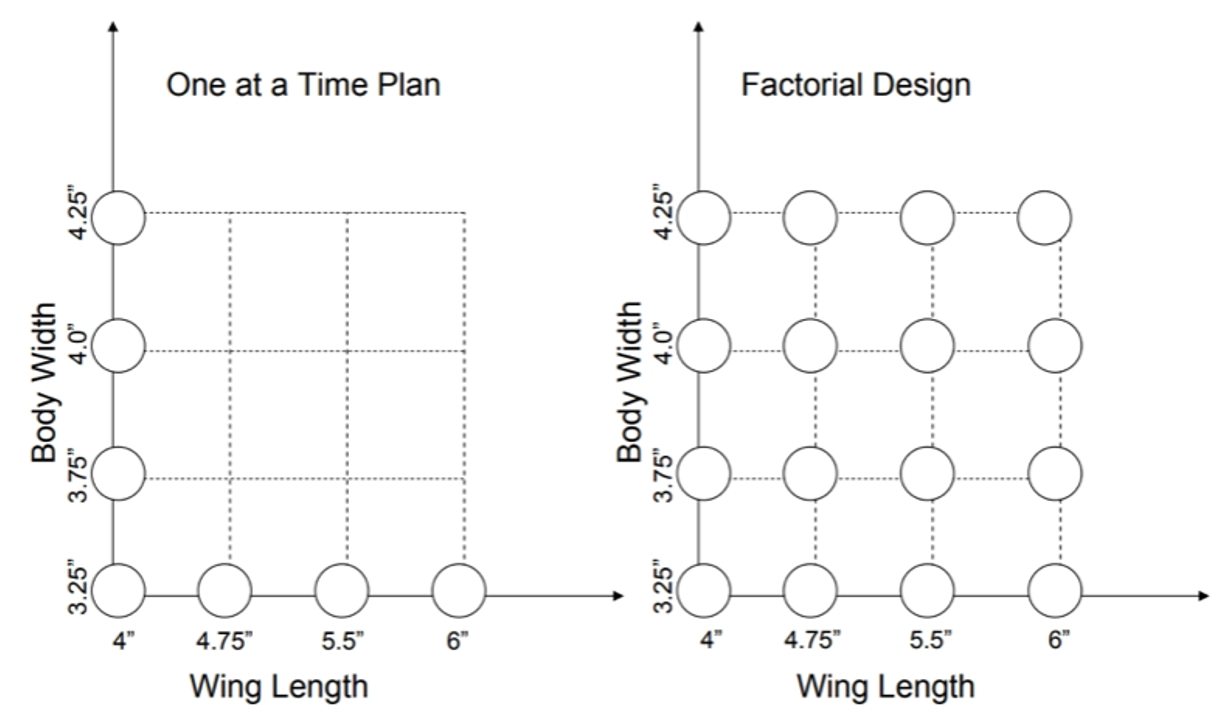
\includegraphics[width=4in]{figures/factorial1.png}
\end{figure}

\end{frame}

\begin{frame}{Factorial designs find better optima}

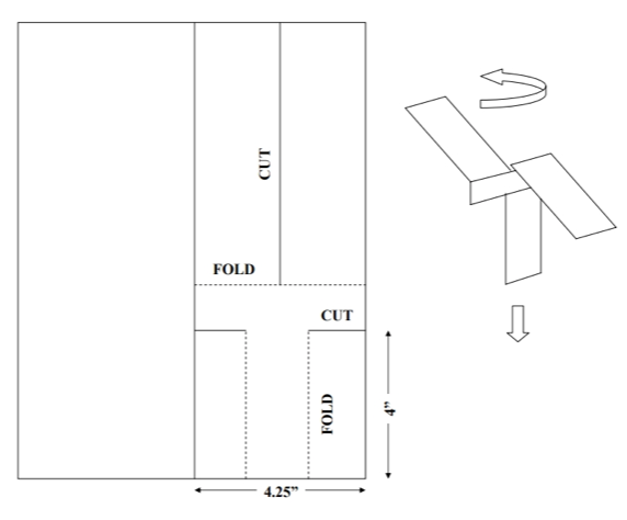
\includegraphics[width=2in]{figures/factorial2-1.png}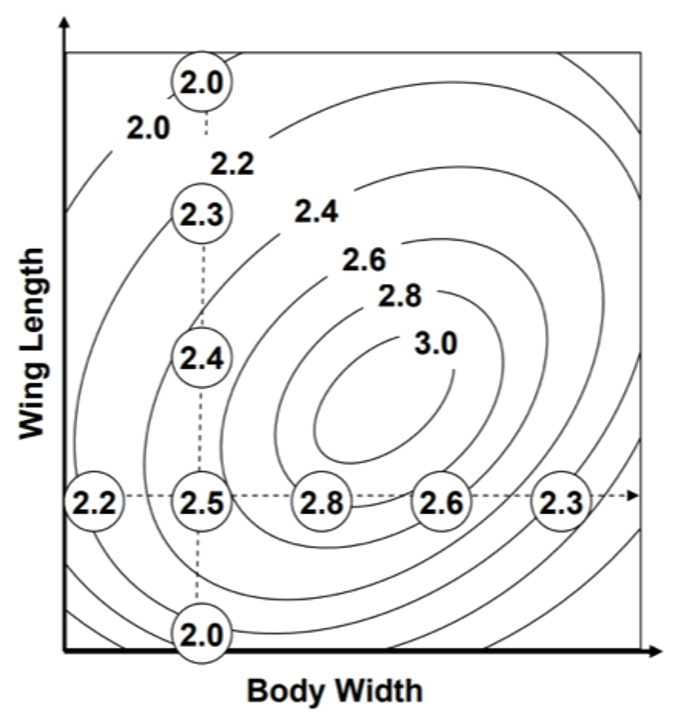
\includegraphics[width=2.5in]{figures/factorial2-3.png}

\end{frame}

\begin{frame}{The problem with OFAT: Interactions}
\centering
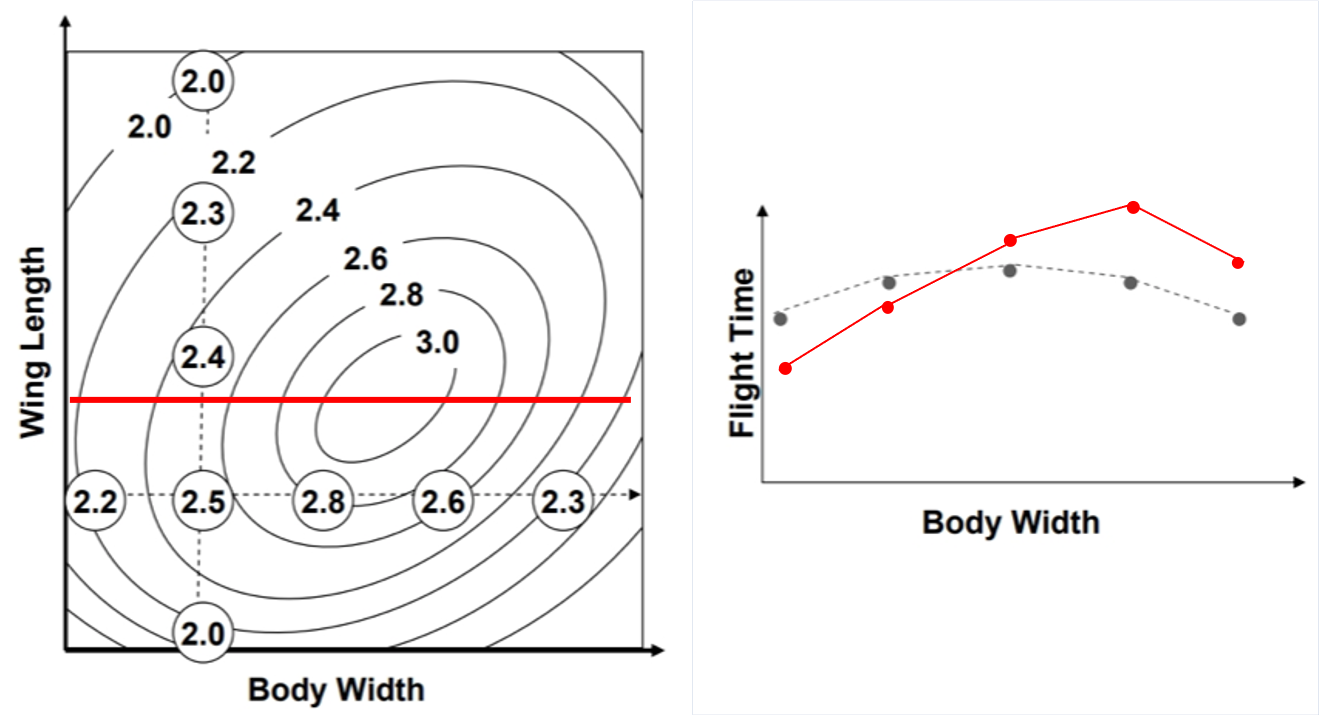
\includegraphics[width=4in]{figures/factorial5.png}

\end{frame}

\begin{frame}{Using interaction plots for diagnosis}
\centering
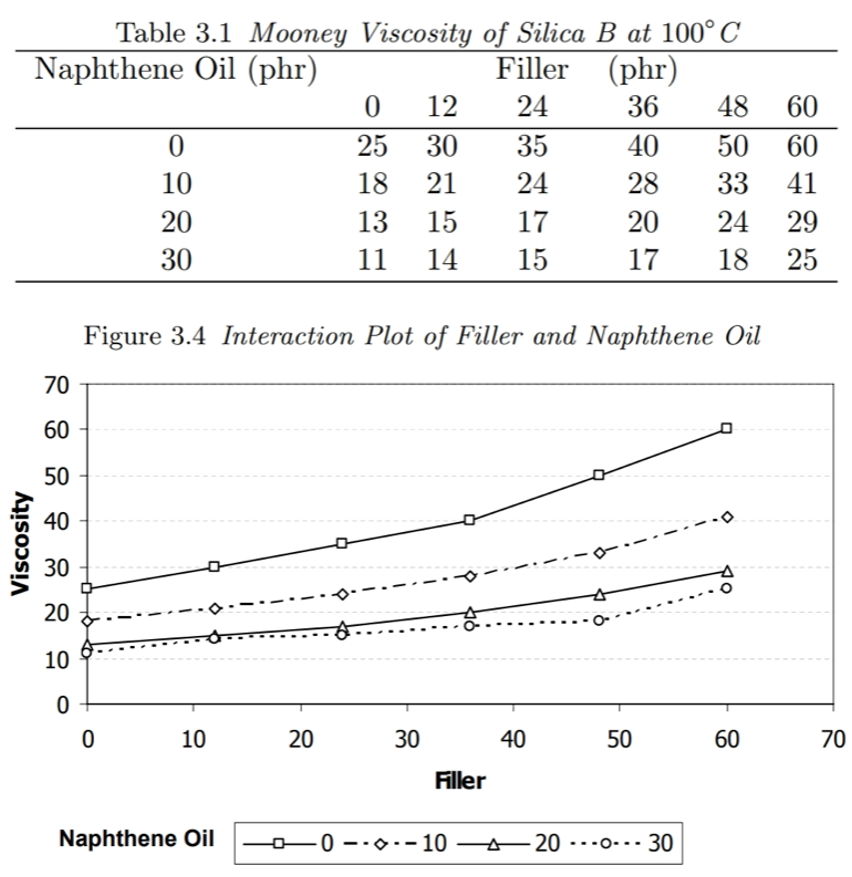
\includegraphics[width=3in]{figures/factorial6.png}

\end{frame}

\begin{frame}{Why do we use factorial designs?}

\begin{itemize}
\item
  Factorial designs find better optima.
\item
  \textbf{Factorial designs are more efficient.}
\item
  Factorial designs make better estimates of effect sizes.
\end{itemize}

\end{frame}

\begin{frame}{Factorial designs seem \emph{less} efficient\ldots{}}

Imagine an experiment with four factors, each with two levels (\(-\),
\(+\)). We want three replicates for each level.

\medskip

One Factor at a Time Design

\begin{itemize}
\item
  3 runs at level (\(-\))
\item
  4 factors \(\times\) 3 runs at (\(+\)) = 12 runs
\item
  \textbf{15 total runs}
\end{itemize}

Factorial Design

\begin{itemize}
\item
  \textbf{$2^4 = \textbf{16}$ total runs}
\end{itemize}

\end{frame}

\begin{frame}{\ldots{}until you look at the designs}

\begin{columns}

\begin{column}{0.45\textwidth}
\begin{center}
OFAT design
\begin{tabular}{cccc}
$x_1$ & $x_2$ & $x_3$ & $x_4$ \\
\hline
\lo & \lo & \lo & \lo \\
\lo & \lo & \lo & \lo \\
\lo & \lo & \lo & \lo \\
\hi & \lo & \lo & \lo \\
\hi & \lo & \lo & \lo \\
\hi & \lo & \lo & \lo \\
\lo & \hi & \lo & \lo \\
\lo & \hi & \lo & \lo \\
\lo & \hi & \lo & \lo \\
\lo & \lo & \hi & \lo \\
\lo & \lo & \hi & \lo \\
\lo & \lo & \hi & \lo \\
\lo & \lo & \lo & \hi \\
\lo & \lo & \lo & \hi \\
\lo & \lo & \lo & \hi \\
 \phantom{\lo} & & & \\
\end{tabular}
\end{center}
\end{column}

\begin{column}{0.45\textwidth}
\begin{center}
Factorial design
\begin{tabular}{cccc}
$x_1$ & $x_2$ & $x_3$ & $x_4$ \\
\hline
\lo & \lo & \lo & \lo \\
\hi & \lo & \lo & \lo \\
\lo & \hi & \lo & \lo \\
\hi & \hi & \lo & \lo \\
\lo & \lo & \hi & \lo \\
\hi & \lo & \hi & \lo \\
\lo & \hi & \hi & \lo \\
\hi & \hi & \hi & \lo \\
\lo & \lo & \lo & \hi \\
\hi & \lo & \lo & \hi \\
\lo & \hi & \lo & \hi \\
\hi & \hi & \lo & \hi \\
\lo & \lo & \hi & \hi \\
\hi & \lo & \hi & \hi \\
\lo & \hi & \hi & \hi \\
\hi & \hi & \hi & \hi \\
\end{tabular}
\end{center}
\end{column}

\end{columns}

\end{frame}

\begin{frame}{Factorial designs give more replicates per run}
\protect\hypertarget{factorial-designs-give-more-replicates-per-run}{}

A factorial design in \(n\) variables has \(2^n\) runs, but \(2^{n-1}\)
replicates at each level (\ensuremath{\boldsymbol{-}},
\ensuremath{\boldsymbol{+}}).

\pause
\bigskip

Imagine a design with \(n\) variables at \(k\) levels.

After the initial design, adding another replicate requires

\begin{itemize}
\item
  \(nk\) runs for a OFAT design
\item
  \(\sim k\) runs for a factorial design
\end{itemize}

\end{frame}

\begin{frame}{Why do we use factorial designs?}

\begin{itemize}
\item
  Factorial designs find better optima.
\item
  Factorial designs are more efficient.
\item
  \textbf{Factorial designs make better estimates of effect sizes.}
\end{itemize}

\end{frame}

\begin{frame}{What are the other factors doing when \(x_3\) is high?}

\begin{columns}

\begin{column}{0.45\textwidth}
\begin{center}
OFAT design
\begin{tabular}{cccc}
$x_1$ & $x_2$ & $x_3$ & $x_4$ \\
\hline
\lo & \lo & \lo & \lo \\
\lo & \lo & \lo & \lo \\
\lo & \lo & \lo & \lo \\
\hi & \lo & \lo & \lo \\
\hi & \lo & \lo & \lo \\
\hi & \lo & \lo & \lo \\
\lo & \hi & \lo & \lo \\
\lo & \hi & \lo & \lo \\
\lo & \hi & \lo & \lo \\
\rowcolor{pink} \lo & \lo & \hi & \lo \\
\rowcolor{pink} \lo & \lo & \hi & \lo \\
\rowcolor{pink} \lo & \lo & \hi & \lo \\
\lo & \lo & \lo & \hi \\
\lo & \lo & \lo & \hi \\
\lo & \lo & \lo & \hi \\
 \phantom{\lo} & & & \\
\end{tabular}
\end{center}
\end{column}

\begin{column}{0.45\textwidth}
\begin{center}
Factorial design
\begin{tabular}{cccc}
$x_1$ & $x_2$ & $x_3$ & $x_4$ \\
\hline
\lo & \lo & \lo & \lo \\
\hi & \lo & \lo & \lo \\
\lo & \hi & \lo & \lo \\
\hi & \hi & \lo & \lo \\
\rowcolor{pink} \lo & \lo & \hi & \lo \\
\rowcolor{pink} \hi & \lo & \hi & \lo \\
\rowcolor{pink} \lo & \hi & \hi & \lo \\
\rowcolor{pink} \hi & \hi & \hi & \lo \\
\lo & \lo & \lo & \hi \\
\hi & \lo & \lo & \hi \\
\lo & \hi & \lo & \hi \\
\hi & \hi & \lo & \hi \\
\rowcolor{pink} \lo & \lo & \hi & \hi \\
\rowcolor{pink} \hi & \lo & \hi & \hi \\
\rowcolor{pink} \lo & \hi & \hi & \hi \\
\rowcolor{pink} \hi & \hi & \hi & \hi \\
\end{tabular}
\end{center}
\end{column}

\end{columns}
\end{frame}

\begin{frame}{What do the effect sizes estimate?}

For OFAT designs:
\begin{center}
	 $\beta_i$ is the effect of moving $x_i$ from \lo\ to \hi\ \\ \textbf{while all other factors stay at \lo}.
\end{center}

\pause
\bigskip
For factorial designs:
\begin{center}
	 $\beta_i$ is the effect of moving $x_i$ from \lo\ to \hi\ \\ \textbf{averaged over all other factors at all levels}.
\end{center}
	
\end{frame}

\begin{frame}{Factorial designs are nested}

\begin{columns}

\begin{column}{0.3\textwidth}
\begin{center}
Factorial design
\begin{tabular}{cccc}
$x_1$ & $x_2$ & $x_3$ & $x_4$ \\
\hline
\lo & \lo & \lo & \lo \\
\hi & \lo & \lo & \lo \\
\lo & \hi & \lo & \lo \\
\hi & \hi & \lo & \lo \\
\rowcolor{pink} \lo & \lo & \hi & \lo \\
\rowcolor{pink} \hi & \lo & \hi & \lo \\
\rowcolor{pink} \lo & \hi & \hi & \lo \\
\rowcolor{pink} \hi & \hi & \hi & \lo \\
\lo & \lo & \lo & \hi \\
\hi & \lo & \lo & \hi \\
\lo & \hi & \lo & \hi \\
\hi & \hi & \lo & \hi \\
\rowcolor{pink} \lo & \lo & \hi & \hi \\
\rowcolor{pink} \hi & \lo & \hi & \hi \\
\rowcolor{pink} \lo & \hi & \hi & \hi \\
\rowcolor{pink} \hi & \hi & \hi & \hi \\
\end{tabular}
\end{center}
\end{column}

\begin{column}{0.3\textwidth}
\begin{center}
When $x_3 = \lo$
\medskip
\begin{tabular}{cccc}
$x_1$ & $x_2$ & $x_4$ \\
\hline
\lo & \lo & \lo \\
\hi & \lo & \lo \\
\lo & \hi & \lo \\
\hi & \hi & \lo \\
\lo & \lo & \hi \\
\hi & \lo & \hi \\
\lo & \hi & \hi \\
\hi & \hi & \hi \\
\end{tabular}
\end{center}
\end{column}

\begin{column}{0.3\textwidth}
\begin{center}
When $x_3 = \hi$
\medskip
\begin{tabular}{ccc}
$x_1$ & $x_2$ & $x_4$ \\
\hline
\rowcolor{pink} \lo & \lo & \lo \\
\rowcolor{pink} \hi & \lo & \lo \\
\rowcolor{pink} \lo & \hi & \lo \\
\rowcolor{pink} \hi & \hi & \lo \\
\rowcolor{pink} \lo & \lo & \hi \\
\rowcolor{pink} \hi & \lo & \hi \\
\rowcolor{pink} \lo & \hi & \hi \\
\rowcolor{pink} \hi & \hi & \hi \\
\end{tabular}
\end{center}
\end{column}

\end{columns}	
\end{frame}

\begin{frame}{Rank revisited}

The rank of a matrix quantifies the number of linearly independent rows or columns.

\medskip
The column rank of a matrix is always equal to the row rank.
\[ \mathrm{rank}(\mathbf{X}) = \mathrm{rank}(\mathbf{X}^\mathrm{T}) \]

This limits the rank to be at most the smaller dimension of the matrix.
\[ \mathrm{rank}(\mathbf{X}) \le \min\{m,n\} \quad\mathrm{if}\quad \mathrm{dim}(\mathbf{A}) = m\times n \]

If the above \emph{equality} holds, we say that the matrix is \textbf{full rank}.

\end{frame}

\begin{frame}{Rank and linear modeling}

Each parameter in a linear model requires one independent piece of information.

\medskip
The linear model $\mathbf{y} = \mathbf{X}\mathbf{\beta} + \mathbf{\epsilon}$ is solvable if and only if the design matrix $\mathbf{X}$ is full rank.
\end{frame}

\begin{frame}{Solvability vs.\ power}

A model is solvable if the design matrix is full rank. However, we need ``extra'' rows (degrees of freedom) to estimate the model's uncertainty.

\medskip
Consider the one parameter model $y = \beta x + \epsilon$. 

Given data ($x$,$y$) = (3,6):
\[ \hat{\beta} = x^{-1}y = 2 \]
\pause
Substituting back we see that
\[ \epsilon = y - \hat{\beta} x = 6 - 2\times 3 = 0 \]
With one data point our estimate is always exact!

\pause
Now let's use two data points: ($x$,$y$) = (3,6) and ($x$,$y$) = (4,12).
\[ \hat{\beta} = \begin{pmatrix} 3\\4 \end{pmatrix}^+ \begin{pmatrix} 6\\12 \end{pmatrix} = 2.64 \]
\[ \epsilon_1 = y_1 - \hat{\beta} x = 6 - 2.64\times 3 = -1.92 \]
\[ \epsilon_2 = y_2 - \hat{\beta} x = 12 - 2.64\times 4 = 1.44 \]
\end{frame}

\begin{frame}{What does this mean for factorial designs?}

A full factorial design with $n$ variables has $2^n$ experiments. It also has $2^n$ coefficients (intercept, first-order, and interaction). We can fit a model to a full factorial design but will have no information leftover to estimate the error.

\medskip
We have three options if we want statistical power behind our factorial designs:

\begin{enumerate}
	\item perform replicates of some (or all) runs
	\item only estimate a subset of the $2^n$ coefficients
	\item some combination of 1 \& 2
\end{enumerate}

\pause
\begin{itemize}
	\item For small $n$ designs we perform replicates since there are already few runs and the interactions are probably significant.
	\item For large $n$ designs we drop coefficients for higher order terms since we already have lots of runs and the higher-order interactions are most likely zero.
\end{itemize}
\end{frame}

\begin{frame}{Summary}

Factorial designs produce more information with fewer runs than OFAT designs.
\begin{itemize}
\item Factorial designs find better optima.
\item Factorial designs are more efficient.
\item Factorial designs make better estimates of effect sizes.
\end{itemize}

\pause
\medskip
As the number of factors increases, factorial designs become \textbf{more} efficient.

\medskip
However, the number of runs can be prohibitive, and we rarely need to estimate higher-order interactions.

\pause
\medskip
\textbf{Fractional factorial designs} require fewer runs by purposefully ignoring the higher-order terms.

\end{frame}

\end{document}
